
\section{SIVIA Algorithm}

\vspace{0.3 cm}
	
	\textcolor{blue} {David DUVERGER}
	
	\vspace{0.5 cm}
	
	I will present here the fusion of the paving of the Gascogne Golf, the robots and their erosion. So, it is the resolution of the following mathematical formula:
	
	$$X(t) = G \cap F_{\delta}(X(t-\delta)) \cap g^{-1}([di,\infty])$$
	

\begin{algorithm}
  \caption{SIVIA algorythm}
  \vspace{0.5 cm}
  \textbf{Inputs}% Inputs section
  \begin{algorithmic}[1]
    \STATE Area $X0$
    \STATE Object $France$
    \STATE Object $Erosion$
    \STATE Object $Robots$
  \end{algorithmic}
  \bigskip

  \textbf{Output}% Output section
  \begin{algorithmic}[1]

    \STATE Boxes $France U Robots U Erosion$
    \STATE Boxes $France$
   	\STATE Boxes $Robots U Erosion$
   	\STATE Boxes $Sea$
  \end{algorithmic}
  \bigskip
  
  \textbf{Initialization}% Initialization section
  \begin{algorithmic}[1]
   	\STATE $stack\gets deque([IntervalVector(X0)])$
	\STATE $lf\gets LargestFirst(eps/2.0)$
	\STATE $k\gets 0$ 
	\STATE $BoxesFranceURobotsUErosion\gets []$
	\STATE $BoxesFrance\gets []$
	\STATE $BoxesRobotsUErosion\gets []$
	\STATE $BoxesSea\gets []$
  \end{algorithmic}
  
\end{algorithm}




\newpage

\vfill


\begin{algorithm}
  \caption{SIVIA algorythm (continued)}
  \begin{algorithmic}
	\WHILE{len(stack)}
	
		\vspace{0.3 cm}
	
  		\STATE $X\gets stack.popleft()$
		\STATE $FranceTest\gets France.function(X)$
		\STATE $ErosionTest\gets Erosion.function(X)$ 
		\STATE $RobotsTest\gets Robots.function(X)$

		\vspace{0.3 cm}

  		\textcolor{blue}{//Obtain the 4 corners of each box in pixel:}\
  		 
  		
  		\STATE $i,j\gets France.toPixels(X[0].lb(),X[1].ub())$
		\STATE $i1,j1\gets France.toPixels(X[0].ub(),X[1].ub())$
		\STATE $i2,j2\gets France.toPixels(X[0].ub(),X[1].lb())$ 
		\STATE $i3,j3\gets France.toPixels(X[0].lb(),X[1].lb())$
		\vspace{0.3 cm}
		
	 	\textcolor{blue}{//If we are in the France, robots or erosion:}\
	 	
	 	\IF{FranceTest==IBOOL.IN or ErosionTest == IBOOL.IN or RobotsTest == IBOOL.IN}
     		\STATE $BoxesFranceURobotsUErosion.append([[i,j],[i1,j1],[i2,j2],[i3,j3]]);$
     		\vspace{0.3 cm}
     	
     	\textcolor{blue}{//If we are in the France:}\

	 	 \IF{FranceTest==IBOOL.IN}
     		\STATE BoxesFrance.append([[i,j],[i1,j1],[i2,j2],[i3,j3]]);
	 	\ENDIF
	 	
	 	\vspace{0.3 cm}
	 	
	 	\textcolor{blue}{//If we are in the robots or erosion:}\
	 	 \IF{RobotsTest == IBOOL.IN or ErosionTest == IBOOL.IN}
     		\STATE $BoxesRobotsUErosion.append([[i,j],[i1,j1],[i2,j2],[i3,j3]]);$
	 	 
	
	 	 \ENDIF
	 	 
	 	 \vspace{0.3 cm}
     		
     	\textcolor{blue}{//Else if we are outside all:}\
	 	 \ELSIF{ $FranceTest = IBOOL.OUT and  ErosionTest = IBOOL.OUT and RobotsTest = IBOOL.OUT$}
	 	 \STATE BoxesSea.append([[i,j],[i1,j1],[i2,j2],[i3,j3]]);
	 	 
     	\ELSE
     
     			\IF{$X.maxdiam()\geq eps$}
          			\STATE $(X1, X2)\gets lf.bisect(X)$
          			\STATE $stack.append(X1)$
         			\STATE $stack.append(X2)$
         		\ENDIF
         	
  		\ENDIF
 	 \ENDWHILE 
	
	\vspace{0.3 cm}
	
  \STATE $vibes.axisEqual()$\\
  return BoxesFranceURobotsUErosion,BoxesFrance,BoxesRobotsUErosion,BoxesSea


  \end{algorithmic}
\end{algorithm}

\vfill

\clearpage



\newpage

	With the help of this algorythm we can have a paving of the intersection between the Gascogne Golf, the robots and their erosion. We arrive to obtain the following result:
	

	
	\begin{figure}[!h] 
    \center
    	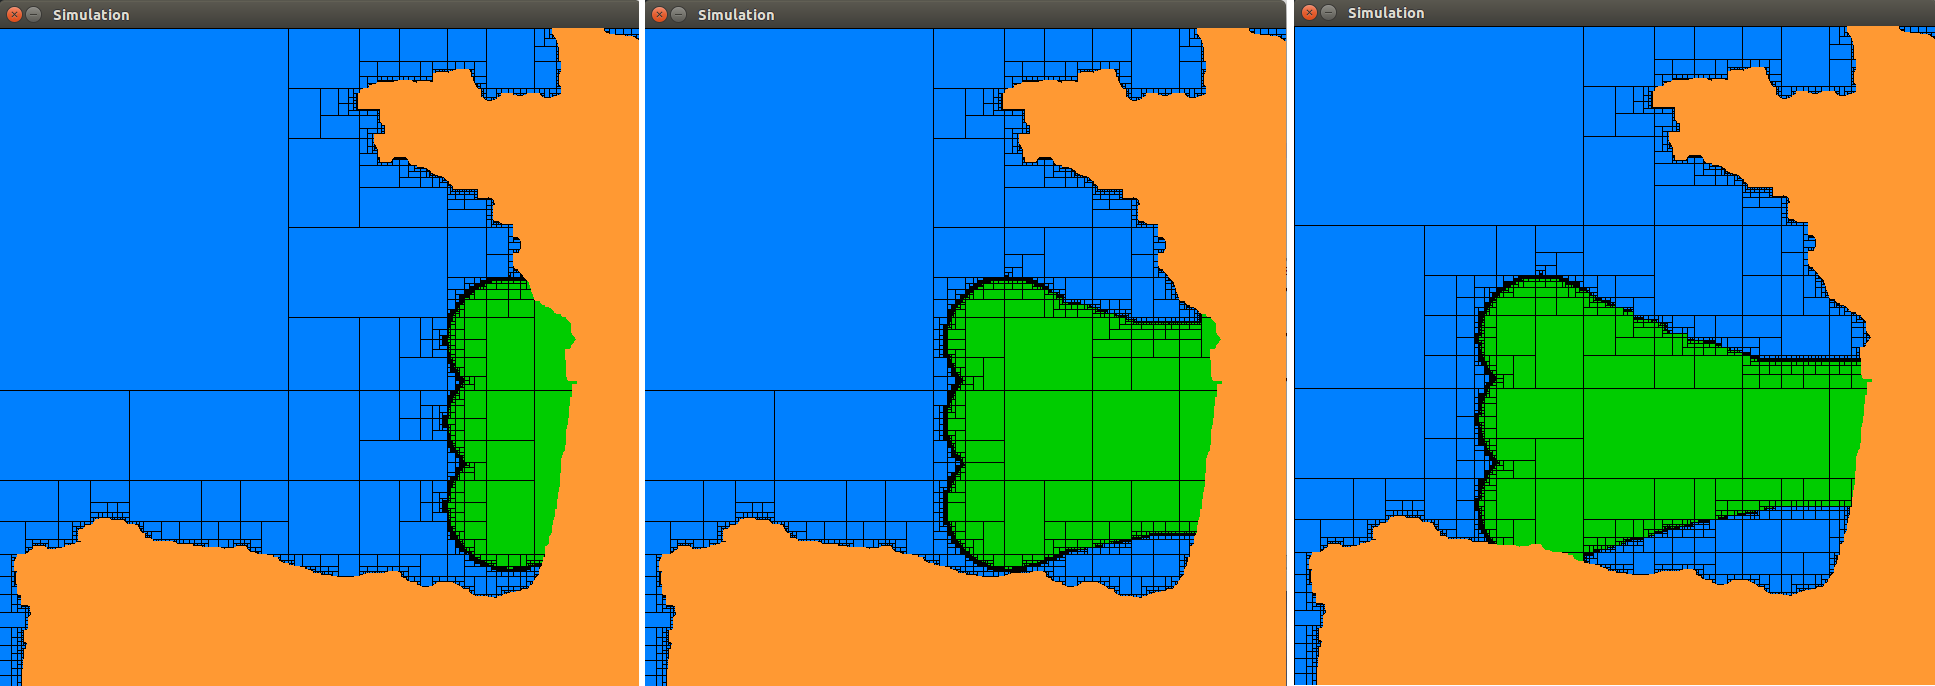
\includegraphics[scale=0.45]{SimulationFusion.png} 
    	\caption{Paving of the intersection between the Gascogne Golf, the robots and their erosion } 
    \label{S1 U S2}
	\end{figure} 
